\section{Auswertung}
\label{sec:Auswertung}

%\begin{figure}
%  \centering
%  \includegraphics{plot.pdf}
%  \caption{Plot.}
%  \label{fig:plot}
%\end{figure}
\subsection{Fourier-Analyse}
Die gemessenen Amplituden werden auf die Amplitude der ersten Oberwelle normiert. Gemessene Amplituden, sowie die Normierung 
dieser ist in \autoref{tab:amplituden} für alle drei Schwingungsformen zu sehen.
\begin{table}[!htp]
\centering
\caption{Amplituden, sowie deren Normierung auf die erste Oberwelle}
\label{tab:amplituden}
\begin{tabular}{c c c c c c c }
\toprule
& \multicolumn{2}{c}{Rechteck} &  \multicolumn{2}{c}{Sägezahn} & \multicolumn{2}{c}{Dreieck} \\
 \cmidrule(lr){2-3} 
  \cmidrule(lr){4-5}
   \cmidrule(lr){6-7}
{n} & {$U_n$ / mV} & {$\frac{U_n}{U_1}$} & {$U_n$ / mV} & {$\frac{U_n}{U_1}$} & {$U_n$ / mV} & {$\frac{U_n}{U_1}$}  \\
\midrule
1 & 2000 & 1.000 & 2160 & 1.000 & 2800  & 1.000  \\
2 & 712 & 0.356  & 1030 & 0.477 & 272 & 0.097 \\
3 & 432 & 0.216  & 656 & 0.304 & 102 & 0.036 \\
4 & 288 & 0.144  & 552 & 0.256 & 50 & 0.018 \\
5 & 216 & 0.108  & 448 & 0.207 & 28 & 0.010 \\
6 & 200 & 0.100  & 384 & 0.178 & 22 & 0.008 \\
7 & 168 & 0.084  & 312 & 0.144 &    &  \\
8 & 144 & 0.072  & 264 & 0.122 &    &  \\
9 & 112 & 0.056  & 248 & 0.115 &    &  \\
10 & 104 & 0.052 & 232 & 0.107 &    &  \\
\bottomrule
\end{tabular}
\end{table}
Die Normierungen werden doppellogarithmisch gegen die Nummer der Oberwellen aufgetragen, worüber anschließend eine lineare
Ausgleichsrechnung durchgeführt wird. Dies ist nötig um die Genauigkeit der Messung hinsichtlich des Abfalls der Oberwellenamplituden
zu überprüfen, da diese mit dem Faktor $\frac{1}{n}$ beziehungsweise $\frac{1}{n^2}$ bei der Dreieckschwinung abnehmen sollen.
Durch eine doppellogarithmische Auftragung und anschließender Bestimmung der Steigung der Ausgleichsgeraden kann diese mit dem 
theoretischen Faktor von $-1$ bei der Rechteck - und Sägezahnschwingung und $-2$ bei der Dreieckschwinung verglichen werden. 
Die Steigung der erechneten Geraden soll bestimmt werden. Bei allen Schwingungsformen wird eine Ausgleichsrechnung der Form 
\begin{equation}
y = a \cdot x + b.
\end{equation} 
durchgeführt, wobei $y$ die Normierung der Amplituden  $\frac{U_n}{U_1}$ ist und  $x$ die Nummer der Oberwellen $n$.
Die Steigung $a$ der Ausgleichsgerade errechnet sich über 
\begin{equation}
\label{eqn:a}
a = \frac {\sum_{i=1}^N (x_i - \overline{x}) (y_i - \overline{y})}{\sum_{i=1}^N (x_i - \overline{x})^2},
\end{equation}
wobei $N$ die Gesamtanzahl der verwendeten Oberwellen ist.
Die aufgetragenen Werte sowie die Ausgleichsgerade zur Rechteckschwingung ist in \autoref{fig:graph_rechteck} zu sehen.
Die Steigung der linearen Ausgleichsgerade zur Rechteckschwingung beträgt nach Gleichung \eqref{eqn:a}
\\ \\
\centerline{$a = ( -1.251 \pm 0.036 ) $.}
\\ \\
\begin{figure}
  \centering
  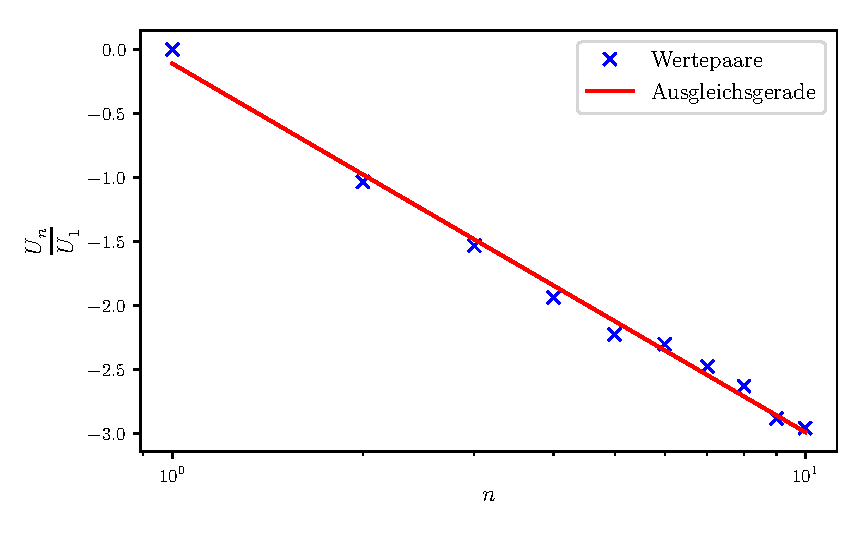
\includegraphics{build/rechteck.pdf}
  \caption{Normierungen der Amplituden der Rechteckschwingung doppellogarithmisch gegen die Nummer der Oberwellen aufgetragen und Ausgleichsgerade.}
  \label{fig:graph_rechteck}
\end{figure}
Bei der Sägezahnschwingung sind die entsprechenden Werte aus \autoref{tab:amplituden}, sowie die zugehörige Ausgleichsgerade
in \autoref{fig:graph_saegezahn} zu sehen. 
Die Steigung der Ausgleichsgerade beträgt mit Gleichung \eqref{eqn:a}
\\ \\ 
\centerline{$ a = (- 0.966 \pm 0.021)$.}
\\ \\
\begin{figure}
  \centering
  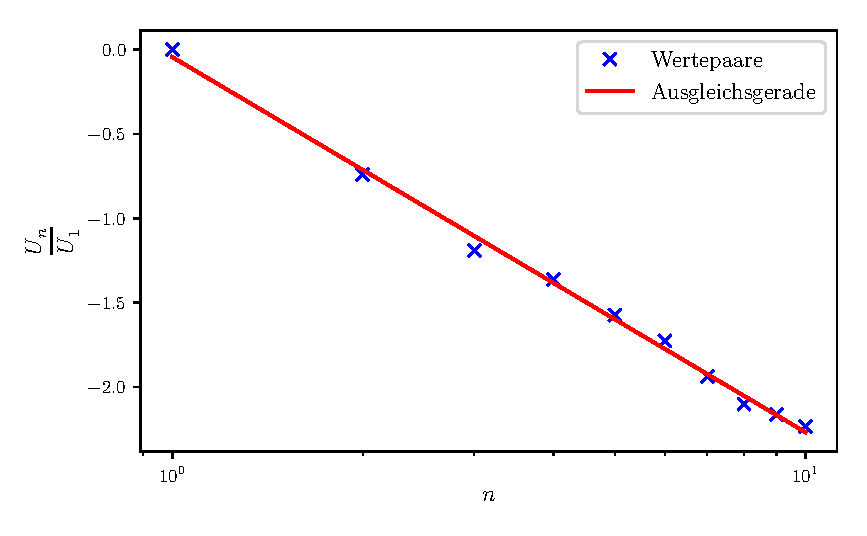
\includegraphics{build/saegezahn.pdf}
  \caption{Normierungen der Amplituden der Sägezahnschwinung doppellogarithmisch gegen die Nummer der Oberwellen aufgetragen und Ausgleichsgerade.}
  \label{fig:graph_saegezahn}
\end{figure}
Statt einer Anzahl von $N = 10$ Oberwellen, liegen hier lediglich $N = 6$ Oberwellen vor (siehe \autoref{sec:Diskussion}).
Die Werte werden entsprechend wieder aus \autoref{tab:amplituden} entnommen und doppellogarithmisch gegen die Anzahl der 
Oberwellen aufgetragen, worüber wieder eine Ausgleichsgerade gebildet wird. Dies ist in \autoref{fig:graph_dreieck} zu sehen.
Die Steigung der Ausgleichsgerade beträgt 
\\ \\
\centerline{$a = ( -2.709 \pm 0.144 )$.}
\\ \\
\begin{figure}
  \centering
  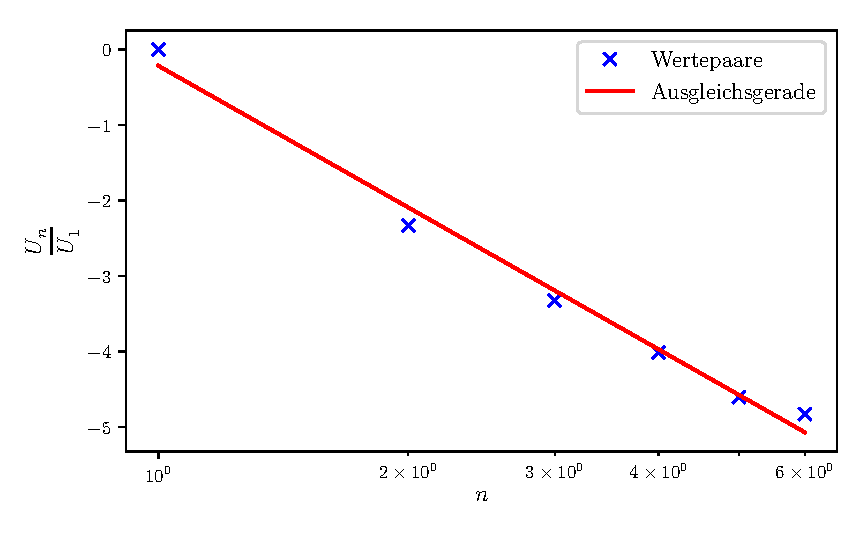
\includegraphics{build/dreieck.pdf}
  \caption{Normierungen der Amplituden der Dreieckschwinung doppellogarithmisch gegen die Nummer der Oberwellen aufgetragen und Ausgleichsgerade.}
  \label{fig:graph_dreieck}
\end{figure}
\newpage
\subsection{Fourier-Synthese}
Die zur Fouriersynthese verwendeten Amplituden sind in \autoref{tab:eingestellt} zu sehen. 
\begin{table}[!htp]
\centering
\caption{Eingestellte Amplituden zur Fouriersynthese zu den drei Schwingungsformen.}
\label{tab:eingestellt}
\begin{tabular}{c c c}
\toprule
 & \multicolumn{2}{c}{Eingestellte Amplituden $U$ / mV } \\
 \cmidrule(lr){2-3}
{Nummer der Oberwelle} & {Reckteck und Sägezahn} & {Dreieck} \\
\midrule
1 & 709.00 & 712.0\\
2 & 354.50 & 178.0\\
3 & 236.30 & 79.1\\
4 & 177.25 & 44.5\\
5 & 141.80 & \\
6 & 118.16 & \\
7 & 101.28 & \\
8 & 88.625 & \\
9 & 78.80  & \\
10 & 70.90 & \\
\bottomrule
\end{tabular}
\end{table}
Bei der Synthese der Rechteckschwingung werden die entsprechenden Werte aus \autoref{tab:eingestellt} entnommen, wobei in die 
Rechteckschwingung nur Oberwellen mit ungerader Nummer einwirken; Oberwellen mit gerader Nummer sind bei der Rechteckschwingung
zu vernachlässigen. Die synthetisierte Funktion ist in \autoref{fig:synth_rechteck} dargstellt.
\begin{figure}
  \centering
  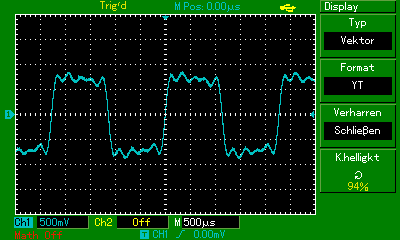
\includegraphics{content/MAP002.png}
  \caption{Synthetisierte Rechteckschwingung.}
  \label{fig:synth_rechteck}
\end{figure}

Bei der Synthese der Sägezahnschwingung werden dieselben Koeffizienten wie bei der Synthese der Rechteckschwingung verwendet, da
die Koeffizienten beider Schwingungsformen mit dem selben Faktor $\frac{1}{n}$ abfallen. Hier wirken allerdings alle 
entsprechende Werte aus \autoref{tab:eingestellt} ein. Die synthetisierte Sägezahnfunktion 
ist in \autoref{fig:synth_saegezahn} zu sehen.
\begin{figure}
  \centering
  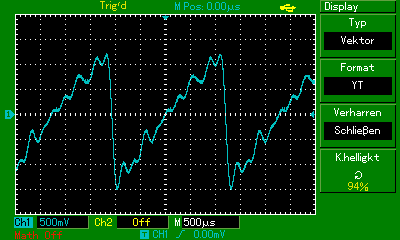
\includegraphics{content/MAP001.png}
  \caption{Synthetisierte Sägezahnschwingung.}
  \label{fig:synth_saegezahn}
\end{figure}

Zur Synthese der Dreieckschwingung werden die entsprechenden Amplituden aus \autoref{tab:eingestellt} verwendet.
Die so synthetisierte Dreieckschwingung ist in \autoref{fig:synth_dreieck} zu sehen.
\begin{figure}
  \centering
  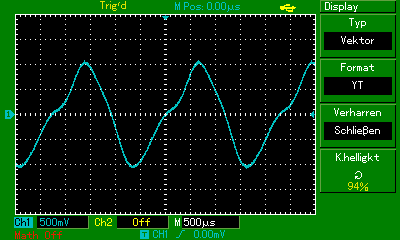
\includegraphics{content/MAP003.png}
  \caption{Synthetisierte Dreieckschwingung.}
  \label{fig:synth_dreieck}
\end{figure}